% Matching Networks Architecture Diagram
% Requires PlotNeuralNet layers (https://github.com/HarisIqbal88/PlotNeuralNet)
\documentclass[border=15pt, multi, tikz]{standalone}
\usepackage{import}
% Uncomment if you have PlotNeuralNet layers
% \subimport{./layers/}{init}
\usetikzlibrary{positioning, shapes.geometric, arrows.meta, calc}

% Define colors for different components
\def\ConvColor{rgb:yellow,5;red,2.5;white,5}
\def\ConvReluColor{rgb:yellow,5;red,5;white,5}
\def\PoolColor{rgb:red,1;black,0.3}
\def\LSTMColor{rgb:blue,5;green,5;white,2}
\def\AttentionColor{rgb:magenta,5;black,2}
\def\SimilarityColor{rgb:orange,5;white,2}
\def\PredictionColor{rgb:green,5;white,3}

\begin{document}
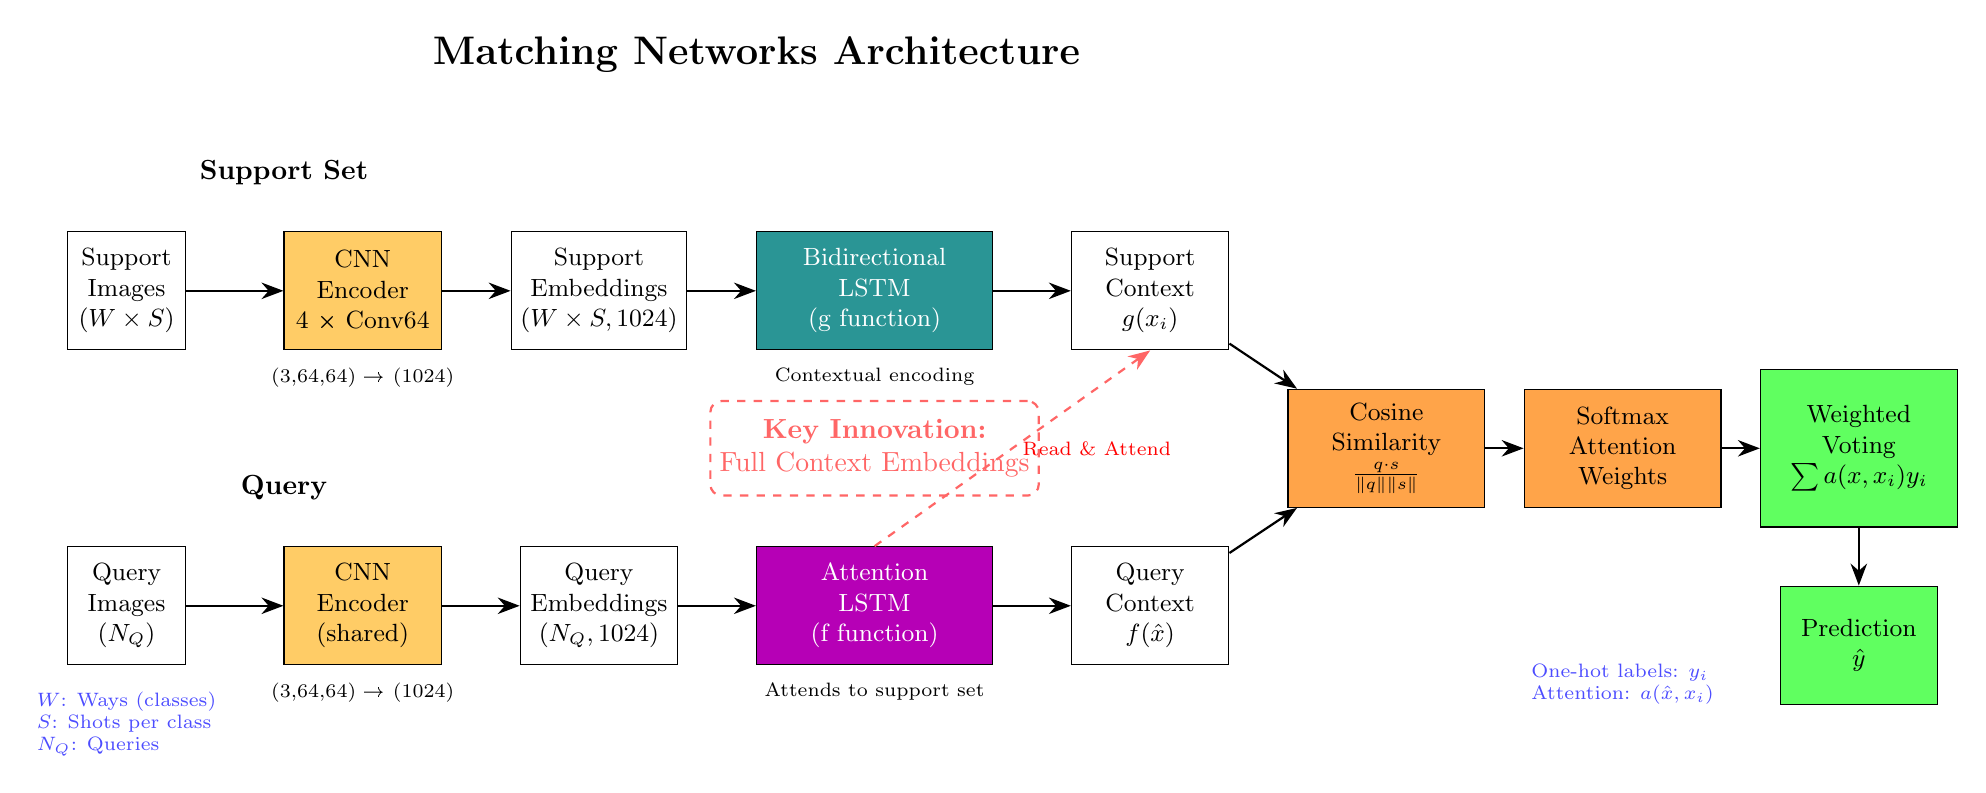
\begin{tikzpicture}[
    box/.style={rectangle, draw, minimum width=2cm, minimum height=1.5cm, align=center, font=\small},
    convbox/.style={box, fill=\ConvColor},
    lstmbox/.style={box, fill=\LSTMColor, text=white},
    attnbox/.style={box, fill=\AttentionColor, text=white},
    simbox/.style={box, fill=\SimilarityColor},
    predbox/.style={box, fill=\PredictionColor},
    arrow/.style={-{Stealth[scale=1.2]}, thick},
    label/.style={font=\footnotesize}
]

%%%%%%%%%%%%%%%%%%%%%%%%%%%%%%%%%%%%%%%%%%%%%%%%%%%%%%%%%%%%%%%%%%%
% Title
%%%%%%%%%%%%%%%%%%%%%%%%%%%%%%%%%%%%%%%%%%%%%%%%%%%%%%%%%%%%%%%%%%%
\node[font=\Large\bfseries] at (0, 8) {Matching Networks Architecture};

%%%%%%%%%%%%%%%%%%%%%%%%%%%%%%%%%%%%%%%%%%%%%%%%%%%%%%%%%%%%%%%%%%%
% Support Set Stream (Top)
%%%%%%%%%%%%%%%%%%%%%%%%%%%%%%%%%%%%%%%%%%%%%%%%%%%%%%%%%%%%%%%%%%%
\node[font=\bfseries] at (-6, 6.5) {Support Set};

% Support images
\node[box, minimum width=1.5cm] (support_img) at (-8, 5) {Support\\Images\\$(W \times S)$};

% CNN Encoder for Support
\node[convbox] (support_cnn) at (-5, 5) {CNN\\Encoder\\4 × Conv64};
\node[label, below=0.1cm of support_cnn] {\scriptsize (3,64,64) → (1024)};

% Support embeddings
\node[box] (support_emb) at (-2, 5) {Support\\Embeddings\\$(W \times S, 1024)$};

% BiLSTM
\node[lstmbox, minimum width=3cm] (bilstm) at (1.5, 5) {Bidirectional\\LSTM\\(g function)};
\node[label, below=0.1cm of bilstm] {\scriptsize Contextual encoding};

% Support context
\node[box] (support_ctx) at (5, 5) {Support\\Context\\$g(x_i)$};

%%%%%%%%%%%%%%%%%%%%%%%%%%%%%%%%%%%%%%%%%%%%%%%%%%%%%%%%%%%%%%%%%%%
% Query Stream (Bottom)
%%%%%%%%%%%%%%%%%%%%%%%%%%%%%%%%%%%%%%%%%%%%%%%%%%%%%%%%%%%%%%%%%%%
\node[font=\bfseries] at (-6, 2.5) {Query};

% Query images
\node[box, minimum width=1.5cm] (query_img) at (-8, 1) {Query\\Images\\$(N_Q)$};

% CNN Encoder for Query (shared)
\node[convbox] (query_cnn) at (-5, 1) {CNN\\Encoder\\(shared)};
\node[label, below=0.1cm of query_cnn] {\scriptsize (3,64,64) → (1024)};

% Query embeddings
\node[box] (query_emb) at (-2, 1) {Query\\Embeddings\\$(N_Q, 1024)$};

% Attention LSTM
\node[attnbox, minimum width=3cm] (attn_lstm) at (1.5, 1) {Attention\\LSTM\\(f function)};
\node[label, below=0.1cm of attn_lstm] {\scriptsize Attends to support set};

% Query context
\node[box] (query_ctx) at (5, 1) {Query\\Context\\$f(\hat{x})$};

%%%%%%%%%%%%%%%%%%%%%%%%%%%%%%%%%%%%%%%%%%%%%%%%%%%%%%%%%%%%%%%%%%%
% Attention Mechanism (Middle)
%%%%%%%%%%%%%%%%%%%%%%%%%%%%%%%%%%%%%%%%%%%%%%%%%%%%%%%%%%%%%%%%%%%

% Attention from Query to Support (dashed line)
\draw[arrow, dashed, color=red!60] (attn_lstm.north) -- 
    node[right, font=\scriptsize, text=red] {Read \& Attend} (support_ctx.south);

%%%%%%%%%%%%%%%%%%%%%%%%%%%%%%%%%%%%%%%%%%%%%%%%%%%%%%%%%%%%%%%%%%%
% Similarity & Prediction (Right)
%%%%%%%%%%%%%%%%%%%%%%%%%%%%%%%%%%%%%%%%%%%%%%%%%%%%%%%%%%%%%%%%%%%

% Cosine Similarity
\node[simbox, minimum width=2.5cm] (cosine) at (8, 3) {Cosine\\Similarity\\$\frac{q \cdot s}{\|q\|\|s\|}$};

% Softmax
\node[simbox, minimum width=2.5cm] (softmax) at (11, 3) {Softmax\\Attention\\Weights};

% Weighted Voting
\node[predbox, minimum width=2.5cm, minimum height=2cm] (voting) at (14, 3) {Weighted\\Voting\\$\sum a(x,x_i)y_i$};

% Final prediction
\node[predbox] (output) at (14, 0.5) {Prediction\\$\hat{y}$};

%%%%%%%%%%%%%%%%%%%%%%%%%%%%%%%%%%%%%%%%%%%%%%%%%%%%%%%%%%%%%%%%%%%
% Connections - Support Stream
%%%%%%%%%%%%%%%%%%%%%%%%%%%%%%%%%%%%%%%%%%%%%%%%%%%%%%%%%%%%%%%%%%%
\draw[arrow] (support_img) -- (support_cnn);
\draw[arrow] (support_cnn) -- (support_emb);
\draw[arrow] (support_emb) -- (bilstm);
\draw[arrow] (bilstm) -- (support_ctx);

%%%%%%%%%%%%%%%%%%%%%%%%%%%%%%%%%%%%%%%%%%%%%%%%%%%%%%%%%%%%%%%%%%%
% Connections - Query Stream
%%%%%%%%%%%%%%%%%%%%%%%%%%%%%%%%%%%%%%%%%%%%%%%%%%%%%%%%%%%%%%%%%%%
\draw[arrow] (query_img) -- (query_cnn);
\draw[arrow] (query_cnn) -- (query_emb);
\draw[arrow] (query_emb) -- (attn_lstm);
\draw[arrow] (attn_lstm) -- (query_ctx);

%%%%%%%%%%%%%%%%%%%%%%%%%%%%%%%%%%%%%%%%%%%%%%%%%%%%%%%%%%%%%%%%%%%
% Connections - Similarity & Prediction
%%%%%%%%%%%%%%%%%%%%%%%%%%%%%%%%%%%%%%%%%%%%%%%%%%%%%%%%%%%%%%%%%%%
\draw[arrow] (support_ctx) -- (cosine);
\draw[arrow] (query_ctx) -- (cosine);
\draw[arrow] (cosine) -- (softmax);
\draw[arrow] (softmax) -- (voting);
\draw[arrow] (voting) -- (output);

%%%%%%%%%%%%%%%%%%%%%%%%%%%%%%%%%%%%%%%%%%%%%%%%%%%%%%%%%%%%%%%%%%%
% Annotations
%%%%%%%%%%%%%%%%%%%%%%%%%%%%%%%%%%%%%%%%%%%%%%%%%%%%%%%%%%%%%%%%%%%
\node[font=\scriptsize, text=blue!70, align=left] at (-8, -0.5) 
    {$W$: Ways (classes)\\ $S$: Shots per class\\ $N_Q$: Queries};

\node[font=\scriptsize, text=blue!70, align=left] at (11, 0) 
    {One-hot labels: $y_i$\\ Attention: $a(\hat{x}, x_i)$};

%%%%%%%%%%%%%%%%%%%%%%%%%%%%%%%%%%%%%%%%%%%%%%%%%%%%%%%%%%%%%%%%%%%
% Key Innovation Box
%%%%%%%%%%%%%%%%%%%%%%%%%%%%%%%%%%%%%%%%%%%%%%%%%%%%%%%%%%%%%%%%%%%
\node[draw, thick, dashed, color=red!60, rounded corners, 
      minimum width=4cm, minimum height=1.2cm, align=center] at (1.5, 3) 
    {\textbf{Key Innovation:}\\ Full Context Embeddings};

\end{tikzpicture}
\end{document}
